% !TeX root = mos-he.tex

%%%%%%%%%%%%%%%%%%%%%%%%%%%%%%%%%%%%%%%%%%%%%%%%%%%%%%%%%%%%%%%%

\refstepcounter{problem}  % 41. The locomotive problem

%%%%%%%%%%%%%%%%%%%%%%%%%%%%%%%%%%%%%%%%%%%%%%%%%%%%%%%%%%%%%%%%

\begin{prob}{הקצה הקצר של המקל}{}{(The little end of the stick)}

אתה שובר מספר גדול של מקלות זכוכית באורך $1$ לשני חלקים. למקום השבירה התפלגות אחידה לאורך המקל.


\que{1} 
מה התוחלת של אורכו של החלק 
\textbf{הקטן}
יותר?

\que{2} 
מה התוחלת של היחס בין אורכו של החלק הקטן לאורכו של החלק הגדול?
\end{prob}

\solution{}

\ans{1}
ההסתברות שנקודת השבירה היא בצד השמאלי של המקל היא
$1/2$
שהיא גם ההסתברות שהנקודה בצד ימין. החלק הקטן יותר נמצא באותו צד שבו נמצאת נקודת השבירה. התוחלת של נקודת השבירה היא באמצע בין קצה המקל לבין אמצע המקל:
\[
E(\textrm{יותר הקטן אורך}) = \frac{1}{2}\cdot\frac{1}{2}=\frac{1}{4}\,.
\]

\ans{2}
ללא הגבלת הכלליות הנח שנקודת השבירה נמצאת בצד הימני של המקל (איור%
~\ref{f.stick}).
היחס בין החלק הקטן והחלק הגדול הוא
$(1-x)/x$
ויש להשתמש בקבוע נירמול (עמוד%
~\pageref{p.normal})
כי התוחלת מחושבת מעל ל-%
$(1/2,1)$,
מחצית הטווח של
$x$:
\begin{eqn}
E(\textrm{יותר קטן / יותר גדול יחס})&=&\left(\frac{1}{1-(1/2)}\right)\int_{\textstyle\frac{1}{2}}^1 \frac{1-x}{x} \,dx\\
&=& 2\int_{\textstyle\frac{1}{2}}^1 \left(\frac{1}{x} -1\right) \,dx \\
&=& 2 (\ln |x| - x)\left|^{\stackrel{\scriptstyle 1}{\rule{0pt}{4pt}}}_{\textstyle\frac{1}{2}} \right. = 2(0-1 -\ln \textstyle\frac{1}{2}  + \textstyle\frac{1}{2})\approx 0.3863\,.
\end{eqn}%
\begin{figure}[tb]
\begin{center}
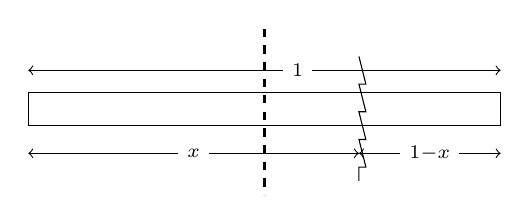
\begin{tikzpicture}
\draw (0,0) -- ++(6,0) -- ++(0,12pt) -- ++(-6,0) -- cycle;
\draw[<->] (0,20pt) --
  node[fill=white,xshift=12pt] {$\scriptstyle 1$} ++(6,0);
\draw[decorate,decoration=saw] (4.2,25pt) -- +(0,-45pt);
\draw[thick,dashed] (3,35pt) -- +(0,-60pt);
\draw[<->] (0,-10pt) --
  node[fill=white] {$\scriptstyle x$} (4.2,-10pt);
\draw[<->] (4.2,-10pt) --
  node[fill=white] {$\scriptstyle 1-x$} (6,-10pt);
\end{tikzpicture}
\end{center}
\caption{שבירת מקל לשני חלקים}\label{f.stick}
\end{figure}

\sml{}
\selectlanguage{english}
\begin{verbatim}
Expectation of length of smaller = 0.2500
Average length of smaller        = 0.2490
Expectation of smaller/larger    = 0.3863
Average smaller/larger           = 0.3845
\end{verbatim}
\selectlanguage{hebrew}

%%%%%%%%%%%%%%%%%%%%%%%%%%%%%%%%%%%%%%%%%%%%%%%%%%%%%%%%%%%%%%%%

\begin{prob}{המקל השבור}{D}{(The broken bar)}

אתה שובר מספר רב של מקלות זכוכית באורך 
$1$
בשתי נדוקות שבירה
(\ref{f.break1}).

\que{1} 
מה התוחלת של אורכו של החלק הקצר ביותר?

\que{2} 
מה התוחלת של אורכו של החלק הארוך ביותר?

\textbf{רמז:}
$x,y$
הם משתנים אקראים בלתי-תלויים בהתפלגות אחידה בתוך 
$(0,1)$.
ניתן להציג כל זוג
$(x,y)$
כנקודה בריבוע
$(0,1)\times (0,1)$ 
(\ref{f.break2}).
מה ההסתברות ש-%
$(x,y) < (.5,.25)$? 

\textbf{:רמז}
עבור 
\quenc{1}
הנח שהחלק השמאלי הוא הקצר ביותר ועבור 
\quenc{2}
הנח שהחלק השמאלי הוא בארוך ביותר.
\begin{figure}[tb]
\centering
\selectlanguage{hebrew}
\subcaptionbox{%
חלוקת מקל לשני חלקים%
\label{f.break1}}
[.45\textwidth]
{
\centering
\begin{tikzpicture}[scale=.75]
\draw (0,0) node[below left] {$0$} --
  ++(6,0) node[below right] {$1$} --
  ++(0,12pt) -- ++(-6,0) -- cycle;
\draw[<->] (0,20pt) --
  node[fill=white] {$\scriptstyle 1$} ++(6,0);
\draw[decorate,decoration=saw] (1.8,25pt) -- +(0,-45pt);
\draw[decorate,decoration=saw] (4.7,25pt) -- +(0,-45pt);
\node[below left] at (1.8,0) {$x$};
\node[below left] at (4.7,0) {$y$};
\path (0,-3.5) rectangle +(0,3.5);
\end{tikzpicture}
}
\hspace{3em}
\subcaptionbox{%
יצוג האורכים במעגל היחידה%
\label{f.break2}}
[.45\textwidth]
{
\centering
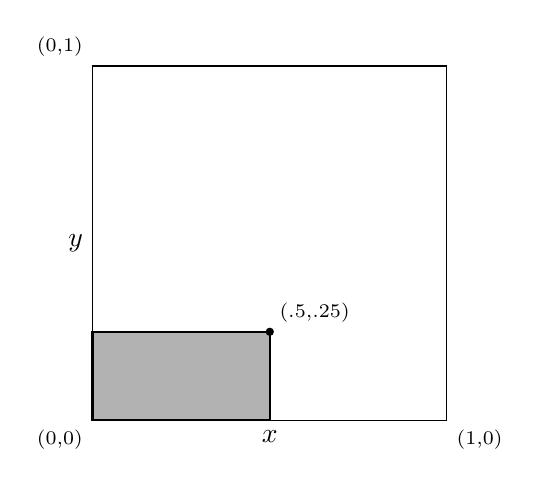
\begin{tikzpicture}[scale=.75]
\draw (-3,-3) rectangle +(6,6);
\draw[thick,fill=white!70!black] (-3,-3) -- ++(0,1.5) -- 
  ++(3,0) -- ++(0,-1.5) -- cycle;
\path (-3,-3) node[below left] {$\scriptstyle (0,0)$} --
  node[below] {$x$} (3,-3)
  node[below right] {$\scriptstyle (1,0)$};
\path (-3,-3) -- node[left] {$y$} (-3,3)
  node[above left] {$\scriptstyle (0,1)$};
\fill (0,-1.5) circle [radius=2pt]
  node[above right] {$\scriptstyle (.5,.25)$};
\end{tikzpicture}
}
\end{figure}
\end{prob}

\solution{}

\ans{1}
ללא הגבלת הכלליות הנח שהחלק השמאלי שאורכו 
$x$
הוא החלק הקצר ביותר. מכאן ש-%
$x<y-x$
ו-%
$x < 1-y$
שניתן לפשט ולקבל
$2x<y$
ו-%
$x+y<1$.

\ref{f.shaded1}
מראה את הקווים
$y=2x$
(אדום) ו-%
$y=1-x$
(כחול). כדי לאמת את אי-השוויונות, 
$(x,y)$
חייבת להיות באיזור באפור לשמאל לשני הקווים. ניתן לחשב את נקודת החיתוך
$(1/2,2/3)$
על ידי פתרון שתי המשוואות.

ניתן לחשב את התוחלת מעל חישוב האינטרגל של המכלפה של
$x$
וההפרש בין שני הקווים. קבוע הנירמול הוא השטח של הריבוע לחלק לשטח של האיזור האפור:
\begin{eqn}
E(x)&=& \frac{1}{1/6}\int_{0}^{1/3} x [(1-x)-2x]\,dx\\
&=&6\int_{0}^{1/3} (x -3x^2)\,dx\\
&=&6\left. \left(\frac{x^2}{2}-x^3\right)\right|_0^{1/3}=\disfrac{2}{18}\approx 0.1111\,.
\end{eqn}%

\begin{figure}[tb]
\centering
\selectlanguage{hebrew}
\subcaptionbox{%
איזור אפור עבור המקל הקצר ביותר%
\label{f.shaded1}}
[.45\textwidth]
{
\centering
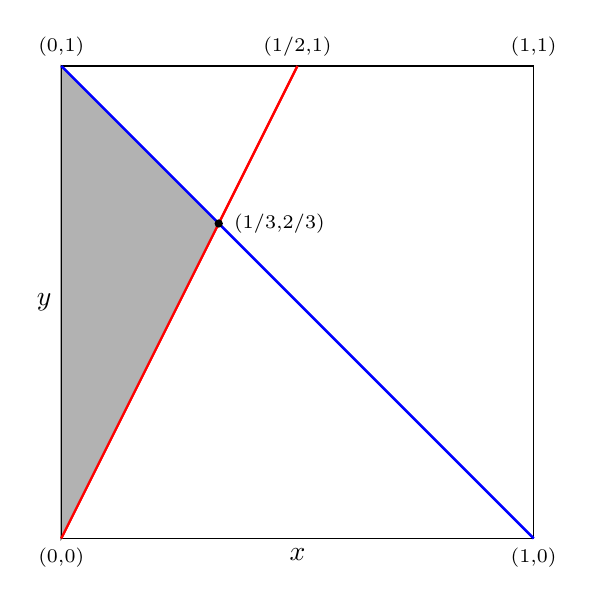
\begin{tikzpicture}[scale=1]
\draw (-3,-3) rectangle +(6,6);
\path (-3,-3) node[below] {$\scriptstyle (0,0)$} --
  node[below] {$x$} (3,-3)
  node[below] {$\scriptstyle (1,0)$};
\path (-3,-3) -- node[left] {$y$} (-3,3)
  node[above] {$\scriptstyle (0,1)$};
\draw[red,thick]  (-3,-3) -- (0,3);
\draw[blue,thick] (-3,3)  -- (3,-3);
\coordinate (P) at (-1,1);
\draw[fill=white!70!black] (-3,-3) -- (P) -- 
  (-3,3) -- cycle;
\draw[red,thick]  (-3,-3) -- (0,3);
\draw[blue,thick] (-3,3)  -- (3,-3);
\fill (P) circle[radius=1.5pt]
  node[right,xshift=2pt] {$\scriptstyle (1/3,2/3)$};
%\draw[thick,dotted] (-3,-3) -- (3,3);
\node[above] at(0,3) {$\scriptstyle (1/2,1)$};
\node[above] at(3,3) {$\scriptstyle (1,1)$};
\end{tikzpicture}
}
\hspace{1em}
\subcaptionbox{%
איזור אפור עבור המקל הארוך ביותר%
\label{f.shaded2}}
[.45\textwidth]
{
\centering
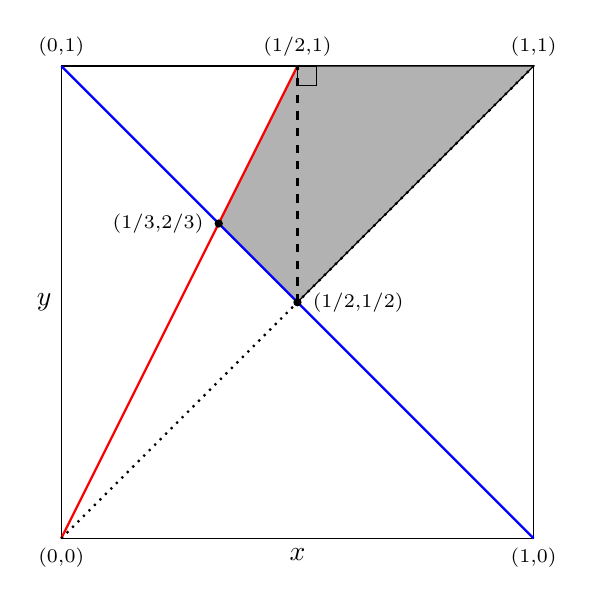
\begin{tikzpicture}[scale=1]
\draw (-3,-3) rectangle +(6,6);
\path (-3,-3) node[below] {$\scriptstyle (0,0)$} --
  node[below] {$x$} (3,-3)
  node[below] {$\scriptstyle (1,0)$};
\path (-3,-3) -- node[left] {$y$} (-3,3)
  node[above] {$\scriptstyle (0,1)$};
\coordinate (P) at (-1,1);
\coordinate (Q) at (0,0);
\draw[fill=white!70!black] (3,3) -- (Q) -- 
  (P) -- (0,3) -- cycle;
\draw[red,thick]  (-3,-3) -- (0,3);
\draw[blue,thick] (-3,3)  -- (3,-3);
\fill (P) circle[radius=1.5pt]
  node[left,xshift=-2pt] {$\scriptstyle (1/3,2/3)$};
\draw[thick,dotted] (-3,-3) -- (3,3);
\fill (Q) circle[radius=1.5pt]
  node[right,xshift=2pt] {$\scriptstyle (1/2,1/2)$};
\node[above] at(0,3) {$\scriptstyle (1/2,1)$};
\node[above] at(3,3) {$\scriptstyle (1,1)$};
\draw[thick,dashed] (Q) -- ++(0,3);
\draw (0,3cm-7pt) rectangle +(7pt,7pt);
\end{tikzpicture}
}
\end{figure}

\ans{2}
כדי שהחלק השמאלי יהיה הארוך ביותר 
$x>y-x$
ו-%
$x>1-y$, 
ולכן
$(x,y)$
חייבת להיות לימינו של
$y=2x$
(אדום) ולימינו של
$y=1-x$
(כחול)
(\ref{f.shaded2}).
בנוסף, לפי ההנחה ש-%
$x$
נמצא לשמאלו של
$y$,
$(x,y)$
חייבת להיות לשמאלו של
$y=x$
(מנוקד).

לפי הליניראיות של התוחלת ניתן לחלק את האיזור האפור לשני משולשים (קו מקווקו) ולחשב את התוחלת בנפרד. קבוע הנירמול הוא השטח של האיזור האפור שהוא
$1/24+1/8=1/6$:
\begin{eqn}
E(\textrm{השמאלי במשולש} \;x)&=& 6\int_{1/3}^{1/2} x [2x-(1-x)]\,dx  \\
&=&6\int_{1/3}^{1/2} \left(3x^2-x\right)\,dx\\
&=&6\left. \left(x^3-\frac{x^2}{2}\right)\right|_{1/3}^{1/2}=\disfrac{1}{9}\\
E(\textrm{הימני במשולש} \;x)&=& 6\int_{1/2}^{1} x (1-x)\,dx\\
&=&6\int_{1/2}^{1} (x-x^2)\,dx\\
&=&6\left. \left(\frac{x^2}{2}-\frac{x^3}{3}\right)\right|_{1/2}^{1}= \disfrac{1}{2}\\
E(x)&=& \disfrac{1}{9}+\disfrac{1}{2} = \disfrac{11}{18}\approx 0.6111\,.
\end{eqn}%

התוחלת של אורכו של החלק הבינוני היא
$1-\frac{2}{18}-\frac{11}{18}=\frac{5}{18}\approx 0.2778$.

\sml{}
\selectlanguage{english}
\begin{verbatim}
Expectations: shortest = 0.1111, middle = 0.2778, longest = 0.6111
Averages:     shortest = 0.1115, middle = 0.2783, longest = 0.6102
\end{verbatim}
\selectlanguage{hebrew}

%%%%%%%%%%%%%%%%%%%%%%%%%%%%%%%%%%%%%%%%%%%%%%%%%%%%%%%%%%%%%%%%

\begin{prob}{לנצח במשחק לא הוגן}{D}{(Winning an unfair game)}

נתון מטבע לא הוגנת שההסתברות להופעת עץ היא 
$1/3 < p < 1/2$,
הטל את המטבע מספר זוגי של פעמים
$N=2n$.
אתה מנצח אם ורק אם 
\textbf{ביותר ממחצית}
ההטלות מופיע עץ.

\que{1}
עבור
$p=\frac{1}{4}, \frac{1}{3}, \frac{1}{2}$,
חשב את
$P_2,P_4,P_6$.
הסבר את הגבלת הבעיה ל-%
$1/3< p < 1/2$.

\que{2}
פתח נוסחה עבור
$P_N$,
ההסתברות לנצח ונוסחה עבור
$T_N$,
ההסתברות לתיקו.

\que{3}
פתח נוסחה עבור ה-%
$N$
עבורו יש את ההסתברות הגבוהה ביותר לנצח.

\textbf{רמז:} 
אם ההסתברות הגבוהה ביותר לנצח היא ב-%
$N$
הטלות אזי 
$P_{N-2} \leq P_N$
ו-%
$P_N\geq P_{N+2}$.
\end{prob}

\solution{}

\ans{1}
ההטלות בלתי-תלויות ולכן נשמתמש בהתפלגות הבינומית:
\begin{eqnarray*}
P_2 &=& p^2\\
P_4 &=& 1\cdot p^4 + \dischoose{4}{1}p^3(1-p)\\
P_6 &=& 1\cdot p^6 + \dischoose{6}{1}p^5(1-p)+\dischoose{6}{2}p^4(1-p)^2\,.
\end{eqnarray*}
עבור
$p=\frac{1}{4}, \frac{1}{3}, \frac{1}{2}$
התוצאות הן:
\[
\begin{array}{r|r|r|r}
\multicolumn{1}{c|}{p}& \multicolumn{1}{c|}{P_2} & \multicolumn{1}{c|}{P_4} & \multicolumn{1}{c}{P_6}\\\hline
1/4 & 1/16=0.0625 & 13/256\approx 0.0501&154/4096\approx 0.0376\\
1/3 & 1/9\approx 0.1111 & 9/81\approx 0.1111&73/729\approx 0.1001\\
1/2 & 1/4=0.2500 & 5/16= 0.3125&22/64\approx 0.3435
\end{array}
\]
הגיוני לשער שכאשר 
$N$
שואף לאינסוף הערכים של
$P_N$
יורדות עבור 
$p=\frac{1}{4}$
ו-%
$p=\frac{1}{3}$
(למרות שקצב הירידה קטן). הערכים של 
$P_N$
עולות עד אחד עבור
$p=\frac{1}{2}$.
לפי רציפות ההסתברות הגדולה ביותר תהיה בטווח
$1/3 < p < 1/2$.

\ans{2} 
כדי לנצח, עץ חייב להופיע ב-%
$i\in\{n+1, n+2, \ldots, 2n-1, 2n=N\}$
הטלות. מההתפלגות הבינומית:
\begin{eqn}
P_N &=& \sum_{i=n+1}^{2n} \dischoose{2n}{i} p^i (1-p)^{2n-i}\\
T_N &=& \dischoose{2n}{n} p^n (1-p)^{n}\,.
\end{eqn}

\ans{3}
כדי שההסתברות עבור
$N=2n$
תהיה הגבוהה ביותר חייב להתקיים:
\[
P_{2n-2} \leq P_{2n} \quad \textrm{ו-} \quad P_{2n}\geq P_{2n+2}\,.
\]
מתי
$P_{2n-2}\not = P_{2n}$?

\textbf{מקרה 1:}
לאחר הטלה
$2n-2$,
עץ הופיע 
$n$
פעמים ופלי
$n-2$
פעמים (כך שהיית מנצח אם היית עוצר כאן), אבל פלי מופיע בשתי ההטלות הבאות. עכשיו יש
$n$
עץ ו-%
$n$
פלי ולכן אתה מפסיד. ההסתברות היא:
\[
\dischoose{2n-2}{n}p^n(1-p)^{n-2} (1-p)^2\,.
\]

\textbf{מקרה $2$:}
לאחר הטלה
$2n-2$,
עץ הופיע 
$n-1$
פעמים ופלי
$n-1$
פעמים (כך שהיית מפסיד אם היית עוצר כאן), אבל עץ מופיע בשתי ההטלות הבאות. עכשיו יש
$n+1$
עץ ו-%
$n-1$
פלי ולכן אתה מנצח. ההסתברות היא:
\[
\dischoose{2n-2}{n-1}p^{n-1}(1-p)^{n-1} p^2\,.
\]
כדי לאמת את
$P_{2n-2}\leq P_{2n}$,
$P_{2n-2}$
לא יכול לגדול כאשר 
$P_{2n}$
נשאר ללא שינוי (מקרה $1$), אבל 
$P_{2n}$
יכול לגדול עד שהיא גבוהה מ-%
$P_{2n-2}$ (מקרה 2).
לכן:
\begin{eqn}
\dischoose{2n-2}{n}p^n(1-p)^{n-2} (1-p)^2 &\leq&
\dischoose{2n-2}{n-1}p^{n-1}(1-p)^{n-1} p^2\\
\disfrac{1}{n} (1-p) &\leq& \disfrac{1}{n-1} p\\
(n-1)(1-p) &\leq& np\\
n &\leq& \disfrac{1-p}{1-2p}\\
2n &\leq& \disfrac{1}{1-2p}+1\,.
\end{eqn}
באופן דומה, כדי לאמת את
$P_{2n}\geq P_{2n+2}$
חייב להיול ש:
\begin{eqn}
\dischoose{2n}{n+1}p^{n+1}(1-p)^{n-1}  (1-p)^2 &\geq&
\dischoose{2n}{n}p^{n}(1-p)^{n}  p^2\\
\disfrac{1}{n+1} (1-p) &\geq& \disfrac{1}{n} p\\
n(1-p)&\geq& (n+1)p\\
n &\geq& \disfrac{p}{1-2p}\\
2n &\geq&\disfrac{1}{1-2p}-1\,.
\end{eqn}
לכן, ערך של
$N=2n$
עבורו מתקבלת ההסתברות הגבוהה ביותר הוא המספר השלם הזוגי הקרוב ביותר ל-%
$1/(1-2p)$.

\sml{}
\selectlanguage{english}
\begin{verbatim}
For probability             = 0.3700
Optimal games to be played  = 4
For  2 games, average won   = 0.1372
For  4 games, average won   = 0.1445
For  6 games, average won   = 0.1431

For probability             = 0.4000
Optimal games to be played  = 6
For  4 games, average won   = 0.1820
For  6 games, average won   = 0.1845
For  8 games, average won   = 0.1680

For probability             = 0.4500
Optimal games to be played  = 10
For  8 games, average won   = 0.2671
For 10 games, average won   = 0.2646
For 12 games, average won   = 0.2640
\end{verbatim}
\selectlanguage{hebrew}

%%%%%%%%%%%%%%%%%%%%%%%%%%%%%%%%%%%%%%%%%%%%%%%%%%%%%%%%%%%%%%%%

\begin{prob}{ממוצע של מספר ההתאמות}{}{(Average number of matches)}

סדר חפיסת קלפים בשורה בסדר הסטנדרטי ואז סדר חפיסה שניה בסדר אקראי מתחת לשורה הראשונה (איור%
~\ref{f.cards}).
מה התוחלת של מספר ההתאמות של קלף בשורה הראשונה עם קלף בשורה מתחתיו?
\end{prob}
\begin{figure}[tb]
\begin{center}
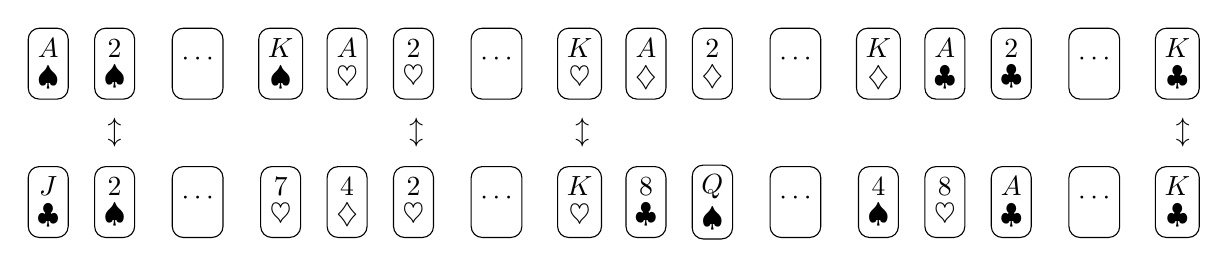
\begin{tikzpicture}
\foreach \x/\v/\s in {
  0/A/\spadesuit,
  1/2/\spadesuit,
  2.25/\cdots/,
  3.5/K/\spadesuit,
  4.5/A/\heartsuit,
  5.5/2/\heartsuit,
  6.75/\cdots/,
  8/K/\heartsuit,
  9/A/\diamondsuit,
  10/2/\diamondsuit,
  11.25/\cdots/,
  12.5/K/\diamondsuit,
  13.5/A/\clubsuit,
  14.5/2/\clubsuit,
  15.75/\cdots/,
  17/K/\clubsuit}
  \node[minimum height=9mm,draw,rounded corners]
    at (\x*24pt,0) {\shortstack{$\v$\\$\s$}};

\foreach \x/\v/\s in {
  0/J/\clubsuit,
  1/2/\spadesuit,
  2.25/\cdots/,
  3.5/7/\heartsuit,
  4.5/4/\diamondsuit,
  5.5/2/\heartsuit,
  6.75/\cdots/,
  8/K/\heartsuit,
  9/8/\clubsuit,
  10/Q/\spadesuit,
  11.25/\cdots/,
  12.5/4/\spadesuit,
  13.5/8/\heartsuit,
  14.5/A/\clubsuit,
  15.75/\cdots/,
  17/K/\clubsuit}
  \node[minimum height=9mm,draw,rounded corners]
    at (\x*24pt,-50pt) {\shortstack{$\v$\\$\s$}};

\node at (24pt,-25pt) {$\updownarrow$};
\node at (133pt,-25pt) {$\updownarrow$};
\node at (193pt,-25pt) {$\updownarrow$};
\node at (410pt,-25pt) {$\updownarrow$};
\end{tikzpicture}
\end{center}
\caption{התאמת שתי חפיסות קלפים}\label{f.cards}
\end{figure}

\solution{}

ההתפלגות אחידה וכלן לכל קלף בשורה השניה אותה המסתברות להתאים לקלף מעליו:
\[
E(\textrm{ההתאמות מספר}) = 52\cdot \frac{1}{52} = 1\,.
\]

\sml{}

\selectlanguage{english}
\begin{verbatim}
Expectation of matches = 1.00
Average of matches     = 1.01
\end{verbatim}
\selectlanguage{hebrew}

%%%%%%%%%%%%%%%%%%%%%%%%%%%%%%%%%%%%%%%%%%%%%%%%%%%%%%%%%%%%%%%%

\begin{prob}{הסתברויות של התאמות}{}{(Probabilities of matches)}

סדר חפיסת קלפים בשורה בסדר הסטנדרטי ואז סדר חפיסה שניה בסדר אקראי מתחת לשורה הראשונה (איור%
~\ref{f.cards}).
פתח נוסחה עבור 
$P(n,r)$,
ההסתברות שיהיו בדיוק 
$r$
התאמות של קלף בשורה הראשונה עם קלף בשורה מתחתיו? הנח ש-%
$P(k,0)$
נתון עבור
$0\leq k\leq n$.
\end{prob}

\solution{}

במבט ראשון נראה שבעיה זו דומה לבעיה%
~$28$
(לתפוס את הזייפן הזהיר) אבל קיים הבדל מהותי. השליפות מהקופסאות הן בלתי-תלויות אבל כאן ההתאמות תלויות אחת בשניה. למשל, אם יש התאמה בקלף הראשון (בהסתברות 
$1/n$),
ההסתברות של התאמה בקלף השני היא
$1/(n-1)$.

ההסתברות שקבוצה 
\textbf{נתונה}
של
$r$
קלפים מתאימות היא:
\begin{equation}\label{eq.r-match}
\disfrac{1}{n}\cdot \disfrac{1}{n-1}\cdot \cdots \cdot \disfrac{1}{n+r-1}\,.
\end{equation}
כדי לקבל בדיוק 
$r$
התאמות, יש להכפיל משוואה%
~\ref{eq.r-match}
ב-%
$P(n-r,0)$,
ההסתברות שאין בכלל התאמות בשאר 
$n-r$
הקלפים. לבסוף, יש 
${n\choose r}$
דרכים לבחור
$r$
התאמות, ולכן:
\begin{eqn}
P(n,r)&=& \dischoose{n}{r}\disfrac{1}{n(n-1)(n+r-1)} P(n-r,0)\\
&=& \disfrac{n!}{r!(n-r)!}\cdot\disfrac{1}{n!/(n-r)!}P(n-r,0)\\
&=&\disfrac{1}{r!}P(n-r,0)\,.
\end{eqn}
נוסחה זו פותרת את הבעיה כי 
$P(k,0)$
נתונה.

\L{Mosteller}
מפתח נוסחה סגורה וגבול עבור
$P(n,r)$:
{
\addtolength{\arraycolsep}{-3pt}
\begin{eqnarray}
P(n,k)&=&\disfrac{1}{k!}\sum_{i=0}^{n-k} \disfrac{(-1)^i}{i!}\\
\label{eq.r-matches-lim}
\lim_{n-r\rightarrow \infty} P(n,k)&\approx& \disfrac{1}{k!}e^{-1}\,.
\end{eqnarray}
}

\sml{}

הרצתי את הסימולציה עבור 
$n=52$
קלפים וחישבתי את ההסתברות ממשוואה%
~\ref{eq.r-matches-lim}.
\selectlanguage{english}
\begin{verbatim}
Probability of 1 matches = 0.3679
Proportion 1 matches     = 0.3710
Probability of 2 matches = 0.1839
Proportion 2 matches     = 0.1828
Probability of 3 matches = 0.0613
Proportion 3 matches     = 0.0569
Probability of 4 matches = 0.0153
Proportion 4 matches     = 0.0168
\end{verbatim}
\selectlanguage{hebrew}

%%%%%%%%%%%%%%%%%%%%%%%%%%%%%%%%%%%%%%%%%%%%%%%%%%%%%%%%%%%%%%%%

\begin{prob}{לבחור את הנדוניה הגדול ביותר}{D}{(Choosing the largest dowry)}

הנח סידרה של 
$n$
קלפים עם הפנים למטה. על פניו של כל קלף נמצא מספר שלם חיובי אבל אין מידע על ההתלפגות שלהם. הפוך את הקלפים אחד-אחד ועיין במספרים. לאחר חשיפת כל אחד מהקלפים אתה יכול להכריז שמספר זה הוא הגדול ביותר בסידרה. אם אתה צודק אתה מנצח אחרת אתה מפסיד.

למשל, אם הסדרה היא 
$(47, 23, 55, 4)$,
אתה מנצח רק אם אתה בוחר שת הקלף השלישי.

בחר קלף לפי אסטרטגיה זו: עבור
$r$
קבוע וותר על
$r-1$
הקלפים הראשונים ובחר את הקלף הראשון שמספרו גדול מכל 
$r-1$
הקלפים.

\que{1}
עבור
$n=4$
ו-%
$r=3$
בדוק את כל התמורות ומצא בכמה מהן את מנצח.

\que{2}
פתח נוסחה עבור ההסתברות לניצחון עבור 
$n, r$
שרירותיים.

\que{3} מצא קירוב להסתברות כאשר 
$n,r\rightarrow \infty$.

\textbf{רמז:}
נתון
$r$
באיזה מקומות יכול להופיע המספר הגדול ביותר
$m$
ובאיזה מקומות המספרים שהם פחות או שווים ל-%
$m$? 

\end{prob}
\solution{}

\ans{1}
כדי לפשט את הסימון נשתמש בדירוג המספרים מנמוך לגבוה
$1,2,\ldots,n$
למרות שהערכים אמיתיים של המספרים לא ידועים.

יש 
$24$
תמורות של ארבעה מספרים. לפי האסטרטגיה אתה מוותר על שני הקלפים הראשונים ובוחר או את הקלף השלישי או את הקלף הרביעי, כך שאתה מפסיד אם $4$ נמצא בשני המקומות הראשונים. מה עם התמורה
$(1,2,3,4)$?
אתה מוותר על
$1,2$
ובוחר 
$3$
בגלל שהוא גובהה יותר מ-%
$1,2$,
אבל אתה מפסיד כי זה לא המספר הגדולה ביותר. מה עם התמורה
$(1,3,2,4)$?
שוב, לפי האסטרטגיה אתה מוותר על
$1,3$,
אבל מוותר גם על
$2$
כי הוא 
\textbf{לא}
גדול מ-%
$1,3$.
כעת אתה בוחר
$4$
ומנצח. נסח טיעונים דומים לכל התמורות ובדוק שכל התמורות עם 
$4$
במסגרת הן נצחונות:
\[
\addtolength{\arraycolsep}{-2pt}
\renewcommand*{\arraystretch}{1.5}
\begin{array}{cc|cc@{\hspace{2em}}cc|cc@{\hspace{2em}}cc|cc@{\hspace{2em}}cc|cc@{\hspace{2em}}cc|cc@{\hspace{2em}}cc|cc}
1&2\;&\;3&4&
1&2\;&\;\fbox{$4$}&3&
1&3\;&\;2&\fbox{$4$}&
1&3\;&\;\fbox{$4$}&2&
1&4\;&\;2&3&
1&4\;&\;3&2\\
2&1\;&\;3&4&
2&1\;&\;\fbox{$4$}&3&
2&3\;&\;1&\fbox{$4$}&
2&3\;&\;\fbox{$4$}&1&
2&4\;&\;1&3&
2&4\;&\;3&1\\
3&1\;&\;2&\fbox{$4$}&
3&1\;&\;\fbox{$4$}&2&
3&2\;&\;1&\fbox{$4$}&
3&2\;&\;\fbox{$4$}&1&
3&4\;&\;1&2&
3&4\;&\;2&1\\
4&1\;&\;2&3&
4&1\;&\;3&2&
4&2\;&\;1&3&
4&2\;&\;3&1&
4&3\;&\;1&2&
4&3\;&\;2&1
\end{array}
\]
ההסתברות לנצח היא
$10/24$.

\ans{2}
אתה מפסיד אם המספר הגדול ביותר נמצא באחד המקומות
$1,\ldots,r-1$.
לכן כדי לנצח המספר הגדול ביותר חייב להיות במקום
$m$
כאשר
$r\leq m\leq n$:
\[
1\quad 2\quad \cdots\quad r-2 \quad r-1 \quad \overbrace{r \quad r+1 \quad \cdots\quad m-1\quad  m \quad m+1\quad \cdots \quad n}^{\textrm{כאן להיות חייב ביותר גדול מספר}}\,.
\]
לפי האסטרטגיה אתה מוותר על
$r-1$
הקלפים הראשונים. אתה תבחר מקום
$m$
אם ורק אם 
\textbf{כל}
במספרים ב-%
$(r,\ldots,m-1)$
קטנים מ%
\textbf{כל}
המספרים ב-%
$(1,\ldots,r)$.
במילים אחרות, המספר הגדול ביותר בסידרה
$(1,\ldots,m-1)$
הוא
\textbf{לא}
בחלק השני של הסידרה
$(r,\ldots m-1)$
אלא בחלק הראשון
$(1,\ldots,r-1)$.
ההסתברות היא:
\[
P((1,\ldots,r-1)\textrm{ב- נמצא}\;(1,\ldots,m-1)\textrm{ב- ביותר הגדול המספר}) = \disfrac{r-1}{m-1}\,.
\]
נביא דוגמה כדי להקל על הבנת הטיעונים. נתון
$1,\ldots,10$
ו-%
$r=5$:
\[
2\quad \quad 5\quad \quad 6\quad \quad 3 \quad \quad  \overbrace{1 \quad \quad 4 \quad \quad 9 \quad \quad 10\quad\quad 8}^{\textrm{כאן נמצא ביותר גדול}}
\]
המספר הגדול ביותר נמצא במקום
$m=9$.
האולם המספר הגדול ביותר ב-%
$(1,\ldots,m-1=8)$
נמצא 
\textbf{בתוך}
הסדרה
$(r=5,\ldots,m-1=8)$
ולכן אתה לא תנצח. לפי האסטרטגיה תבחר
$9$,
המספר הראשון שהוא גדול ביותר מכל המספרים ב-%
$(1,\ldots,r-1=4)$
ותפסיד כי
$10>9$.
לעומת זאת, אם הוחלפו המקומות של
$9$
ו-%
$10$
אזי המספר הגדול ביותר שהוא פחות מ-%
$10$
הוא 
$6$
במקום
$3<r=5$,
ולכן לפי האסטרטגיה לא תבחר ב-%
$1,4$
ותנצח:
\[
\begin{array}{l}
\overbrace{2\quad \quad 5\quad \quad 6\quad \quad 3}^{\textrm{כאן}} \quad \quad  \overbrace{1 \quad \quad 4 \quad \quad \mathbf{9}}^{\textrm{כאן לא}}  \quad \quad 10\quad\quad 8\\
\overbrace{2\quad \quad 5\quad \quad \mathbf{6}\quad \quad 3}^{\textrm{כאן}} \quad \quad  \overbrace{1 \quad \quad 4}^{\textrm{כאן לא}} \quad \quad 10  \quad \quad 9\quad\quad 8
\end{array}
\]
ההסתברות שהמספר הגדול ביותר נמצא ב-%
$m$
הוא
$1/n$
ולכן:
\begin{equation}\label{eq.dowry1}
P(\textrm{ניצחון}) = \sum_{m=r}^{n} \disfrac{1}{n} \cdot \disfrac{r-1}{m-1}= \disfrac{r-1}{n}\sum_{m=r}^{n} \disfrac{1}{m-1}\,.
\end{equation}
עבור
$n=4, r=3$,
$P(\textrm{ניצחון}) = 5/12=
10/24$,
התוצאה שמצאנו על ידי בדיקת כל התמורות.

\ans{3}
נכתוב את משוואה%
~\ref{eq.dowry1}
כך:
\begin{equation}\label{eq.dowry2}
P(\textrm{ניצחון}) =\disfrac{r-1}{n}\left(\sum_{m=2}^{n} \disfrac{1}{m-1}-\sum_{m=2}^{r-1} \disfrac{1}{m-1}\right)\,.
\end{equation}
עבור 
$n,r$
גדולים ניתן למצוא קירוב לשתי הסדרות ההרמוניות במשוואה%
~\ref{eq.dowry2}
כך:
\begin{equation}\label{eq.dowry3}
P(\textrm{ניצחון})=\disfrac{r}{n}(\ln n - \ln r)=\disfrac{r}{n}\ln \disfrac{n}{r}=-\disfrac{r}{n}\ln \disfrac{r}{n}\,.
\end{equation}
נסמן
$x=r/n$
ונמצא את המקסימום מהנגזרת:
\begin{eqn}
(-x\ln x)' &=& -x\cdot \frac{1}{x} + (-1) \ln x=0\\
\ln x &=& -1\\
x &=& 1/e\,.
\end{eqn}
לכן כדי למקסם את ההסתברות לנצח בחר
$r \approx n/e$,
וממשוואה%
~\ref{eq.dowry3}:
\[
P(\textrm{ניצחון})\approx-\disfrac{1}{e}\ln\left(\disfrac{1}{e}\right)=\disfrac{1}{e}\approx \disfrac{1}{3}\,,
\]
גבוהה הרבה יותר מהסתברות
$1/n$
לנצח על ידי בחירת קלף אקראי.

\sml{}

הרצתי את הסימולציה עם
$100$
קלפים וערכי
$r$
קרובים ל-%
$100/e$:
\selectlanguage{english}
\begin{verbatim}
Reject cards before r = 36:
Probability of wins   = 0.3674
Proportion wins       = 0.3641
Reject cards before r = 37:
Probability of wins   = 0.3678
Proportion wins       = 0.3759
Reject cards before r = 38:
Probability of wins   = 0.3679
Proportion wins       = 0.3548
Reject cards before r = 30:
Probability of wins   = 0.3590
Proportion wins       = 0.3601
\end{verbatim}
\selectlanguage{hebrew}

%%%%%%%%%%%%%%%%%%%%%%%%%%%%%%%%%%%%%%%%%%%%%%%%%%%%%%%%%%%%%%%%

\begin{prob}{בחירת המספר האקראי הגדול ביותר}{D}{\\(Choosing the largest random number)}

הנח סידרה של 
$n$
קלפים עם הפנים למטה. על פניו של כל קלף נמצא מספר ממשי עם התפלגות אחידה ב-%
$[0.0,1.0]$.
הפוך את הקלפים אחד-אחד ועיין במספרים. לאחר חשיפת כל אחד מהקלפים, אתה יכול להכריז שמספר זה הוא הגדול ביותר בסידרה. אם אתה צודק אתה מנצח אחרת אתה מפסיד.

השתמש באסטרטגיה של בעיה%
~$47$:
עבור
$r$
קבוע וותר על 
$r-1$
הקלפים הראשונים ובחר את הקלף הראשון שגדול מהמספר הגדול ביותר ב-%
$r-1$
קלפים הראשונים.

\textbf{הגדרה:}
$d$,
\textbf{ערך שווה-נפש},
הוא הערך שמתחתיו אתה מוותר על הקלף ומעליו אתה בחור את הקלף.

\que{1} 
חשב את
$d$
עבור
$n=1$
וחשב את ההסתברות לנצח.

\que{2}
חשב את
$d$
עבור
$n=2$
וחשב את ההסתברות לנצח.

\que{3}
חשב את
$d$
עבור
$n=3$.
אל תנסה לחשב את ההסתברות לנצח!

\textbf{הערה:}
בבעיה%
~$47$
הערכים יכולים להיות
$100, 200, 300$ 
או
$100, 50, 20$
כך שחשיפת המספר הראשון לא מספק מידע על המספרים האחרים. בבעיה זו ההתלפגות אחידה ולכן אם המספר הראשון הוא 
$0.3$
ההסתברות שהמספר השני יהיה גדול יותר היא 
$0.7$.
\end{prob}

\solution{}

יהי
$v_1,v_2,v_3$
המספרים על שלושת קלפים.

\ans{1}
אין ברירה אלא לבחור את הקלף הראשון כי אין קלפים אחרים. לכן אין ערך שווה-נפש.
$v_1$
הוא המספר "הגדול ביותר" ו-%
$P(\textrm{ניצחון})=1$.

\ans{2}
אם אתה בוחר את הקלף הראשון
$P(\textrm{ניצחון})=v_1$
שהיא ההסתברות שהמספר על הקלף השני קטן יותר. אם אתה מוותר על הקלף הראשון,
$P(\textrm{ניצחון})=1-v_1$
שהיא ההסתברות ש-%
$v_2>v_1$.
לכן, אם 
$v_1<0.5$ 
בחר את הקלף השני כי
$1-v_1>0.5$
ואם 
$v_1>0.5$
בחר את הקלף הראשון. מכאן ש-%
$d=0.5$.

נוסחה לחישוב ההסתברות לנצח:
\begin{equation}\label{eq.largest-random1}
P(\textrm{ניצחון}) = P(\textrm{ניצחון} \,|\,v_1<0.5)\,P(v_1<0.5)+ P(\textrm{ניצחון}\,|\,v_1>0.5)\,P(v_1>0.5)\,.
\end{equation}
$P(v_1<0.5)=0.5$
נובע מההתפלגות האחידה. מה עם
$P(\textrm{ניצחון} \,|\,v_1<0.5)$? 
לפי האסטרטגיה אתה מנצח אם
$0.5<v_2<1$
אבל גם אם
$v_1<v_2<0.5$.
ההתפלגות של 
$v_1$
היא אחידה ב-%
$(0,0.5)$
ולכן  ההסתברות ש-%
$v_1<v_2<0.5$
היא מחצית הטווח:
\[
P(\textrm{ניצחון} \,|\,v_1<0.5)=\disfrac{1}{2} + \disfrac{1}{4}=\disfrac{3}{4}\,.
\]
מחישוב דומה עבור
$v_1>0.5$
ומשוואה%
~\ref{eq.largest-random1}
מתקבל:
\[
P(\textrm{ניצחון})=\disfrac{3}{4}\cdot\disfrac{1}{2}+\disfrac{3}{4}\cdot\disfrac{1}{2}=\disfrac{3}{4}\,.
\]

\ans{3}
אם אתה בוחר את הקלף הראשון,
$P(\textrm{ניצחון})=v_1^2$
כי הקלף השני והשלישי חייבים להיות קטנים מהראשון.

אם אתה מוותר על הקלף הראשון ובוחר את השני כי 
$v_2>v_1$
אזי:
\begin{itemize}
\item $P(\textrm{ניצחון})=v_1(1-v_1)$
אם
$v_2<v_1$
(וותר על
$v_2$)
ו-%
$v_3>v_1$
(בחר את 
$v_3$
ותנצח).
\item $P(\textrm{ניצחון})=(1-v_1)v_1$
אם
$v_2>v_1$ 
(בחר את
$v_2$)
ו-%
$v_3<v_1$
(תנצח כי
$v_3<v_2$).
\item $P(\textrm{ניצחון})=\frac{1}{2}(1-v_1)^2$
אם
$v_2>v_1$
(בחר את
$v_2$)
ו-%
$v_3>v_1$.
הגורם
$1/2$
לוקח בחשבון שניצחון תלוי ביחס:
$v_3<v_2$
(ניצחון) או
$v_2<v_3$
(הפסד).
\end{itemize}

הערך שווה-נפש 
$d$
הוא ערך עבורו ההסתברות לנצח על ידי בחירת הקלף הראשון שווה להסתברות לנצח על ידי ויתור על הקלף הראשון:
\begin{eqn}
d^2 &=& 2d(1-d) + \frac{1}{2}(1-d)^2\\
5d^2 - 2d -1 &=&0\\
d&=& \disfrac{1+\sqrt{6}}{5}\approx 0.6899\,.
\end{eqn}
\L{Gilbert\&Mosteller \cite[page~55]{gilbert}}
מראים שעבור
$n=3$:
\[
P(\textrm{ניצחון}) = \disfrac{1}{3}+\disfrac{d}{2}+\disfrac{d^2}{1}-\disfrac{3d^3}{2}\approx 0.6617\,.
\]

\newpage

\sml{}

\selectlanguage{english}
\begin{verbatim}
For  3 cards:
Indifference value = 0.6000
Probability of win = 0.6693
Proportion of wins = 0.6628
Indifference value = 0.6899
Probability of win = 0.6617
Proportion of wins = 0.6711
Indifference value = 0.7200
Probability of win = 0.6519
Proportion of wins = 0.6473
\end{verbatim}
\selectlanguage{hebrew}

%%%%%%%%%%%%%%%%%%%%%%%%%%%%%%%%%%%%%%%%%%%%%%%%%%%%%%%%%%%%%%%%

\begin{prob}{להכפיל את הדיוק}{}{(Doubling your accuracy)}

נתון שני מקלות באורכים
$L_1<L_2$
ומכשיר למדידת אורך ששגיאת המדידה שלו ניתן על ידי התפלגות נורמלית %
\footnote{בעיה זו מניחה שהקורא מכיר התלפגויות נורמליות.}
עם ממוצע
$0$
ושונות
$\sigma^2$.
ניתן למדוד את אורכי המקלות על ידי מדידת כל מקל בנפרד. האם יש דרך מדוייקת יותר?
\end{prob}

\solution{}

\begin{figure}[bt]
\begin{center}
\begin{tikzpicture}
\draw (0,0) -- ++(6,0) -- ++(0,12pt) -- ++(-6,0) -- cycle;
\draw[<->] (0,24pt) --
  node[fill=white] {$\scriptstyle L_1+L_2$} ++(14,0);
\draw (6,0) -- ++(8,0) -- ++(0,12pt) -- ++(-8,0) -- cycle;
\begin{scope}[yshift=-48pt]
\draw (0,0) -- ++(8,0) -- ++(0,12pt) -- ++(-8,0) -- cycle;
\draw[yshift=12pt] (0,0) -- ++(0,12pt) -- ++(6,0) -- ++(0,-12pt);
\draw[<->] (6,20pt) --
  node[fill=white] {$\scriptstyle L_2-L_1$} ++(2,0);
\end{scope}
\end{tikzpicture}
\end{center}
\caption{מדידת האורכים של שני מקלות}\label{f.rods}
\end{figure}
הנח את המקלות קצה לקצה ומדד
$L_s=L_1+L_2$
ואחר כך הנח אותם צד לצד ומדד
$L_d=L_2-L_1$ (איור%
~\ref{f.rods}).
חשב
$L_1,L_2$:
\begin{eqn}
\textstyle\frac{1}{2}(L_s-L_d)=\frac{1}{2}((L_1+L_2)-(L_2-L_1))&=&L_1\\
\textstyle\frac{1}{2}(L_s+L_d)=\frac{1}{2}((L_1+L_2)+(L_2-L_1))&=&L_2\,.
\end{eqn}
השגיאות במדידות הן
$e_s, e_d$
כך שהשגיאות התוצאות הן:
\begin{eqn}
\textstyle\frac{1}{2}((L_s+e_s)-(L_d+e_d))&=&L_1+\textstyle\frac{1}{2}(e_s-e_d)\\
\textstyle\frac{1}{2}((L_s+e_s)+(L_d+e_d))&=&L_2+\textstyle\frac{1}{2}(e_s+e_d)\,.
\end{eqn}
ממוצע של השגיאות במכשיר הוא
$0$
ולכן הממוצע של שתי המדידות גם כן $0$. השונות יורדת למחצית מערכה הקודמת:%
\footnote{%
המדידות בלתי-תלויות ולכן הקווריאנס הוא $0$.}
\begin{eqn}
\mathrm{Var}\left(\textstyle\frac{1}{2}\left(e_s-e_d\right)\right)&=&
  \textstyle\frac{1}{4}(\sigma^2+(-1)^2\sigma^2)=\frac{1}{2}\sigma^2\\
\mathrm{Var}\left(\textstyle\frac{1}{2}(e_s+e_d)\right)&=&
  \textstyle\frac{1}{4}( \sigma^2+\sigma^2)=\frac{1}{2}\sigma^2\,.
\end{eqn}%

\sml{}

\selectlanguage{english}
\begin{verbatim}
For L1 = 40, L2 = 16, variance = 0.50:
L1 mean = 39.9907, L1 variance = 0.2454
L2 mean = 16.0030, L2 variance = 0.2520

For L1 = 40, L2 = 16, variance = 1.00:
L1 mean = 39.9934, L1 variance = 0.4949
L2 mean = 15.9889, L2 variance = 0.4878

For L1 = 40, L2 = 16, variance = 2.00:
L1 mean = 39.9924, L1 variance = 0.9940
L2 mean = 16.0104, L2 variance = 1.0069
\end{verbatim}
\selectlanguage{hebrew}
הממוצעים מדוייקים מאוד והשונויות יורדות למחצית מערכן הקודמת עבור 
$\sigma^2=0.5,\sigma^2=1.0$
אבל השונות לא מושפעות עבור
$\sigma^2=2.0$.

%%%%%%%%%%%%%%%%%%%%%%%%%%%%%%%%%%%%%%%%%%%%%%%%%%%%%%%%%%%%%%%%

\begin{prob}{משוואות ריבועיות אקראיות}{}{(Random quadratic equations)}

תהי 
$x^2+2bx+c=0$
משוואה ריבועית המוגדרת מעל
$[-B,B]\times[-B,B]$
עבור
$B\geq 1$.

\que{1}
מה ההסתברות שהשורשים ממשיים?

\que{2} 
כאשר 
$B\rightarrow \infty$
מה ההסתברות שהשורשים ממשיים?
\end{prob}

\solution{}

\ans{1}
השורשים יהיו ממשיים אם הדיסקרימיננט 
$4b^2-4c\geq 0$
לא-שלילי. איור%
~\ref{f.real-roots}
מראה גרף של הפרבולה
$c=b^2$
כאשר השורשים המרוכבים נמצא בשטח האפור. למשל, עבור
$(b,c)=(1,2)$, 
ל-%
$x^2+2x+2$
שורשים מרוכבים (נקודה אדומה) ועבור
$(b,c)=(2,2)$
ל-%
$x^2+4x+2$
שורשים ממשיים (נקודה כחולה).

\begin{figure}[tb]
\begin{center}
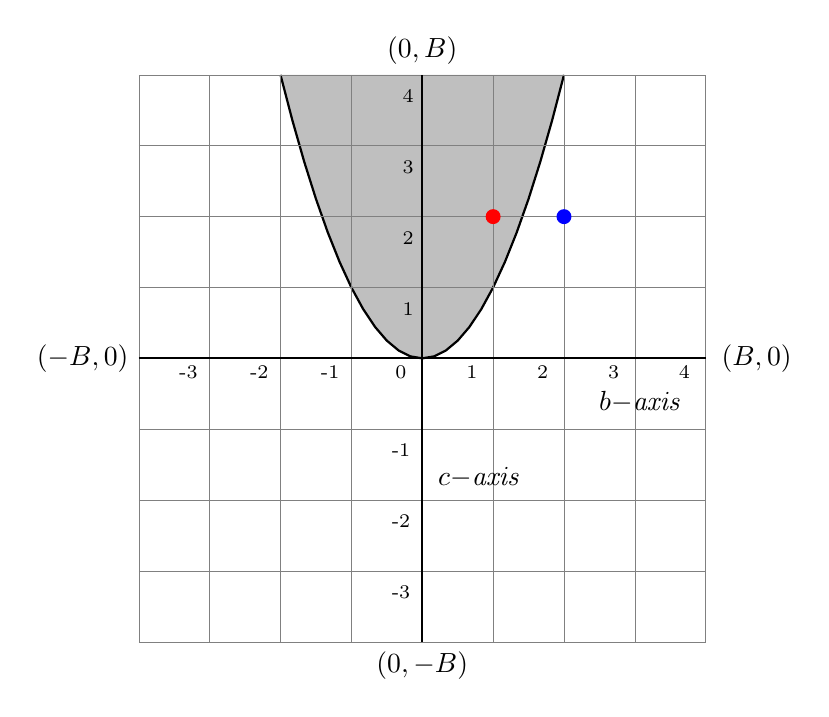
\begin{tikzpicture}[scale=.9]
\fill [white!50!gray, domain=-2:2]
      (-2, 4) -- plot ({\x}, {\x*\x}) -- (2, 4) -- cycle;
\draw [thick, domain=-2:2]
      (-2, 4) -- plot ({\x}, {\x*\x}) -- (2, 4);
\draw[help lines] (-4,-4) grid (4,4);
\draw[thick] (-4,0) -- (4,0);
\draw[thick] (0,-4) -- (0,4);
\foreach \x in {-3,...,4}
  \node at (\x-.3,-.2) {\scriptsize \x};
\foreach \y in {1,...,4}
  \node at (-.2,\y-.3) {\scriptsize \y};
\foreach \y in {-3,...,-1}
  \node at (-.3,\y-.3) {\scriptsize \y};
\draw[thick] (0,-4) node[below] {$(0,-B)$} -- 
  node[right,near start,xshift=2pt,yshift=8pt]
  {$c\mathit{-axis}$} (0,4) node[above] {$(0,B)$};
\draw[thick] (-4,0) node[left] {$(-B,0)$} --
  node[below,very near end,xshift=2pt,yshift=-8pt] 
  {$b\mathit{-axis}$} (4,0) node[right,xshift=2pt] {$(B,0)$};
\fill[red] (1,2) circle(3pt);
\fill[blue] (2,2) circle(3pt);
\end{tikzpicture}
\end{center}
\caption{%
עבור 
$(b,c)$
בשטח האפור השורשים של
$x^2+2bx+c$
מרוכבים}
\label{f.real-roots}
\end{figure}

נחשב את השטח האפור על ידי אינטגרציה:
\[
\int_{-\sqrt{B}}^{\sqrt{B}} (B-b^2)\,db=
\left. Bb-\disfrac{b^3}{3}\right|_{-\sqrt{B}}^{\sqrt{B}}=
\left(B^{3/2}-\frac{B^{3/2}}{3}\right)-
\left(-B^{3/2}+\frac{B^{3/2}}{3}\right)=
\disfrac{4}{3}B^{3/2}\,.
\]
השטח הכולל של
$[-B,B]\times[-B,B]$
הוא
$4B^2$
ולכן:
\begin{eqn}
P(\textrm{מרוכבים שורשים})&=&\disfrac{\frac{4}{3}B^{3/2}}{4B^2}=\disfrac{1}{3\sqrt{B}}\\
P(\textrm{ממשיים שורשים})&=&1-\disfrac{1}{3\sqrt{B}}\,.
\end{eqn}
\ans{2}
\[
\lim_{B\rightarrow\infty}
P(\textrm{ממשיים שורשים})=
\lim_{B\rightarrow\infty} \left(1-\disfrac{1}{3\sqrt{B}}\right)=
1\,.
\]

\sml{}
\selectlanguage{english}
\begin{verbatim}
For B =  4:
Probability of real roots = 0.8333
Proportion real roots     = 0.8271
For B = 16:
Probability of real roots = 0.9167
Proportion real roots     = 0.9205
For B = 64:
Probability of real roots = 0.9583
Proportion real roots     = 0.9582
\end{verbatim}
\selectlanguage{hebrew}

%%%%%%%%%%%%%%%%%%%%%%%%%%%%%%%%%%%%%%%%%%%%%%%%%%%%%%%%%%%%%%%%

\begin{prob}{הילוך מקרי דו-ממדי}{}{(Two-dimensional random walk)}

חלקיק נמצא במרכז של מערכת צירים דו-ממדית. החלקיק צועד ימינה או שמאלה על ציר ה-%
$x$
עם הסתברות 
$1/2$
לכל כיוון 
\textbf{ובו-זמנית}
צועד למעלה או למטה על ציר ה-%
$y$
עם הסתברות 
$1/2$
לכל כיוון. איור%
~\ref{f.2d-random-walk}
מראה הילוך מקרי של 
$22$
צעדים שמתחיל ונגמר במרכז.

\que{1}
מה ההסתברות שהחלקיק חוזר למרכז ב-$2$ צעדים?

\que{2}
פתח נוסחה עבור התוחלת של מספר הביקורים של ההחלקיק במרכז.

\que{3}
השתמש בקירוב של
\L{Stirling}
כדי לקבל הערכה של התוחלת של מספר הביקורים של ההחלקיק במרכז עבור $n$ גדול.

\textbf{רמז:}
השתמש במשתנה מסמן כדי לחשב את התוחלת.
\begin{figure}[t]
\begin{center}
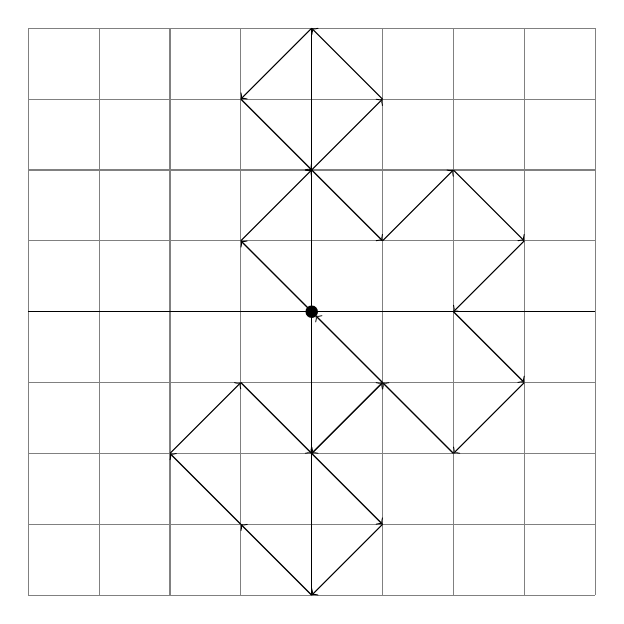
\begin{tikzpicture}[scale=.9]
\draw[color=gray] (-4,-4) grid (4,4);
\draw (-4,0) -- (4,0);
\draw (0,-4) -- (0,4);
\fill (0,0) circle[radius=2.5pt];
\draw[->] (0,0)  -- (-1,1);
\draw[->] (-1,1) -- (0,2);
\draw[->] (0,2)  -- (1,3);
\draw[->] (1,3)  -- (0,4);
\draw[->] (0,4)  -- (-1,3);
\draw[->] (-1,3) -- (0,2);
\draw[->] (0,2)  -- (1,1);
\draw[->] (1,1)  -- (2,2);
\draw[->] (2,2)  -- (3,1);
\draw[->] (3,1)  -- (2,0);
\draw[->] (2,0)  -- (3,-1);
\draw[->] (3,-1) -- (2,-2);
\draw[->] (2,-2) -- (1,-1);
\draw[->] (1,-1) -- (0,-2);
\draw[->] (0,-2) -- (1,-3);
\draw[->] (1,-3) -- (0,-4);
\draw[->] (0,-4) -- (-1,-3);
\draw[->] (-1,-3)-- (-2,-2);
\draw[->] (-2,-2)-- (-1,-1);
\draw[->] (-1,-1)-- (0,-2);
\draw[->] (0,-2) -- (1,-1);
\draw[->] (1,-1) -- (.055,-.055);
\end{tikzpicture}
\end{center}
\caption{הילוך מקרי דו-ממדי}\label{f.2d-random-walk}
\end{figure}
\end{prob}

\solution{}

\ans{1}
הנקודות באיור%
~\ref{f.two-moves}
מראות את המקומות האפשריים בהם החלקיק יכול להיות לאחר שני צעדים:
\begin{itemize}
\item
המסלול הירוק מראה איך להגיע ל-%
$(\pm 2, \pm 2)$
על ידי שני צעדים באותו כיוון. ההסתברות היא
$\left(\frac{1}{4}\right)^2= \frac{1}{16}$.
\item
המסלול האדום מראה איך להגיע ל-%
$(\pm 2,0)$
או ל-%
$(0,\pm 2)$.
יש שני מסלולים אפשריים לכל נקודה ולכן ההסתברות היא
$2\cdot\left(\frac{1}{4}\right)^2= \frac{2}{16}$.
\item
המסלול הכחול מראה איך להגיע ל-%
$(\pm 1,\pm 1)$
וחזרה למרכז. ההסבתרות היא
$\frac{1}{16}$.
\end{itemize}
נסמן ב-%
$P_{2n}(x,y)$
ההסתברות שהחלקיק מגיע ל-%
$(x,y)$
ב-%
$2n$
צעדים.

ארבעת המסלולים הכחולים האפשריים הם היחידים שחוזרים למרכז ולכן:
\[
P_{2}(0,0)=\frac{4}{16}\,.
\]
\begin{figure}[tb]
\begin{center}
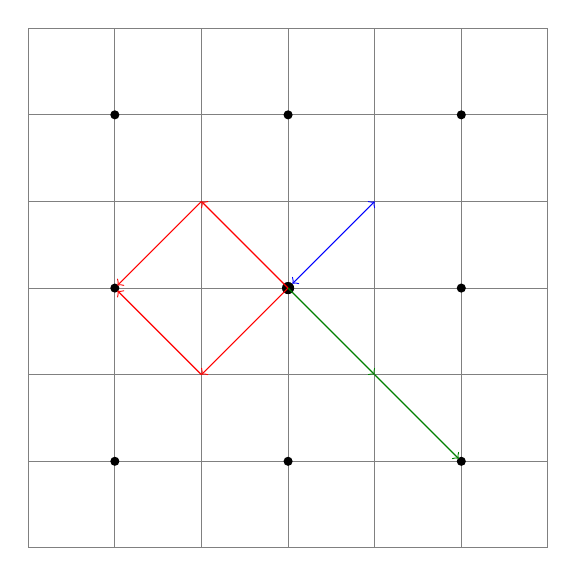
\begin{tikzpicture}[scale=1.1]
\draw[color=gray] (-3,-3) grid (3,3);
\fill (0,0) circle[radius=2pt];
\foreach \x/\y in {2/2, 2/-2, -2/2, -2/-2, 
                   0/2, 0/-2, 2/0, -2/0}
  \fill (\x,\y) circle[radius=1.5pt];
\draw[->,red] (0,0) -- (-1,-1);
\draw[->,red] (-1,-1) -- (-1.97,-.03);
\draw[<-,red] (-1.97,0.03) -- (-1,1);
\draw[<-,red] (-1,1) -- (0,0);
\draw[->,green!50!black] (0,0) -- (1,-1);
\draw[->,green!50!black] (1,-1) -- (1.97,-1.97);
\draw[<->,blue] (.05,.05) -- +(.95,.95);
%\draw[->,blue] (-0.1,0) -- +(1,1);
%\draw[->,blue] (1.1,1) -- +(-1,-1);
\end{tikzpicture}
\end{center}
\caption{שני צעדים בהילוך מקרי}\label{f.two-moves}
\end{figure}
\ans{2}
בחירת הכיוון בשני מצירים היא בלתי-תלויה:
\begin{equation}\label{eq.2d-1}
P_{2n}(0,0) = P_{2n}(0,b) \cdot P_{2n}(a,0) \,,
\end{equation}
כאשר 
$a,b$
הם מספרים שלמים שרירותיים.

החלקיק יחזור למרכז אם ורק אם בשני הצירים מספר הצעדים 
$+1$
שווה המספר צעדים
$-1$.
יש 
${2n \choose n}$
דרכים לסדר
$n$
צעדים של
$+1$
ו-%
$n$
צעדים של
$-1$
ולכן:
\begin{eqnlabels}
\nonumber{}P_{2n}(0,b) =P_{2n}(a,0)&=&
\dischoose{2n}{n}\left(\disfrac{1}{2}\right)^n\left(\disfrac{1}{2}\right)^{n}\\
\label{eq.return-to-origin1}P_{2n}(0,0) &=&
\left[\dischoose{2n}{n}\left(\disfrac{1}{2}\right)^{2n}\right]^2\,.
\end{eqnlabels}%
הגדר משתנים מסמנים
$I_{2n}(0,0)$
לחזרה למרכס ב-%
$2n$
צעדים ותהי
$E(0,0)$
התוחלת של
\textbf{מספר החזרות למרכז}
במספר כלשהו של צעדים. ניתן לחשב:
\[
E(0,0) = \sum_{n=1}^{\infty}E(I_{2n}(0,0))\,.
\]
אפשר לשאול מה קורה אם החלקיק צעד שלושה צעדים וחזרה למרכז ושוב צועד שלושה צעדים וחזור למרכז. האם ערכו של
$I_6(0,0)$ 
צריך להיות שניים ולא אחד? התשובה היא שהחזרה השניה מתרחשת ב-%
$12$
צעדים וייספר על ידי
$I_{12}(0,0)=1$.

ממשוואות%
~\ref{eq.expectation-prob},~\ref{eq.expectation-sum}:
\begin{equation}
E(0,0) =
\sum_{n=1}^{\infty}E(I_{2n}(0,0)) =
E\left(\sum_{n=1}^{\infty}I_{2n}(0,0)\right) =
\sum_{n=1}^{\infty}P_{2n}(0,0) =
\sum_{n=1}^{\infty}\left[\dischoose{2n}{n}\left(\disfrac{1}{2}\right)^{2n}\right]^2\,.\label{eq.return-to-origin2}
\end{equation}


\ans{3}
לפי הקירוב של
\L{Stirling}
$n! \approx \sqrt{2\pi n}\left(n/e\right)^n$:
\begin{eqnlabels}
\nonumber{}E_{2n}(0,0) &=&
\left[\dischoose{2n}{n}
\left(\disfrac{1}{2}\right)^{2n}\right]^2 \\
\nonumber{}&=&
\left[\disfrac{(2n)!}{(n!)^2}
\left(\disfrac{1}{2}\right)^{2n}\right]^2 \\
\nonumber{}&\approx&
\left(\disfrac{1}{2}\right)^{4n}
\disfrac{(\sqrt{2\pi \cdot 2n})^2
         \left(2n/e\right)^{4n}}
        {(\sqrt{2\pi n})^{4}
         \left(n/e\right)^{4n}} \\
\nonumber{}&=&\left(\disfrac{1}{2}\right)^{4n}\disfrac{4\pi n}{4\pi^2 n^2}\cdot
\disfrac{\left(n/e\right)^{4n}\cdot 2^{4n}}{\left(n/e\right)^{4n}}\\
\nonumber{}&=& \disfrac{1}{\pi n}\\
\label{eq.rw-2d}E(0,0) &=& \disfrac{1}{\pi}\sum_{n=1}^{\infty}\disfrac{1}{n}\,,
\end{eqnlabels}%
שהיא סידרה הרמונית שמתבדרת, כלומר, עם הסתברות 
$1$
החלקיק חוזר למרכז!

בגלל ש-%
$E(0,0)=\infty$
מספר הפעמים שהחלקיק חוזר למרכז לא חסום. אולם, לפי האקסיומה הראשונה של הסתברות
(עמוד%
~\pageref{p.first-axiom}), $P(0,0)$,
ההסתברות שהחלקיק יחזור למרכז חייבת להיות\
$0\leq P(0,0) \leq 1$
ולכן
$P(0,0)=1$
שמשמעותה היא שבוודאות החלקיק חוזר למרכז. באופן כללי, התוחלת של משתנה אקראי היא אינסופית אם ורק אם ההסתברות היא אחד.

\sml{}

הרצתי את הסימולציה 
$100$
עם מיליון צעדים בכל אחת.

\selectlanguage{english}
\begin{verbatim}
Proportion returned to origin = 0.8700
\end{verbatim}
\selectlanguage{hebrew}

ההסתברות שהחלקיק יחזור למרכז היא 
$1$
ולכן התוצאה אמורה להיות קרוב ל-%
$1.0000$.
המשמעות של התוצאה שקיבלתי היא שלמרות שהחלקיק יחזור למרכז, מספר הצעדים יכול להיות מאוד מאוד גדול.

%%%%%%%%%%%%%%%%%%%%%%%%%%%%%%%%%%%%%%%%%%%%%%%%%%%%%%%%%%%%%%%%

\begin{prob}{הילוך מקרי תלת-ממדי}{D}{(Three-dimensional random walk)}

חלקיק נמצא במרכז של מערכת צירים תלת-ממדית. החלקיק צועד ימינה או שמאלה על ציר ה-%
$x$
עם הסתברות 
$1/2$
לכל כיוון,
\textbf{ובו-זמנית}
צועד למעלה או למטה על ציר ה-%
$y$
עם הסתברות 
$1/2$
לכל כיוון,
\textbf{ובו-זמנית}
צועד פנימה או החוצה על ציר ה-%
$z$
עם הסתברות 
$1/2$
לכל כיוון.

\que{1}
פתח נוסחה עבור התוחלת של מספר הפעמים שהחלקיק חוזר למרכז והשתמש בקירוב של 
\L{Stirling}
כדי להעריך את ערכה.

\textbf{רמז:}
פתח נוסחה להסתברות ואחר כך השתמש במשתנה מסמן.

\que{2}
מה ההסתברות שהחלקיק יחזור למרכז
\textbf{לפחות פעם אחת}?

\textbf{רמז:}
השתמש בשיטה של בעיה%
~$4$.
\end{prob}

\solution{}

$P_{2n}$,
ההסתברות לחזור למרכז לאחר
$2n$
צעדים, נתון על ידי הכללת משוואה%
~\ref{eq.2d-1}
לשלושה ממדים:
\begin{equation}\label{eq.rw-multiply}
P_{2n} =
P_{2n}(x=0\textrm{ל- חוזר})\,P_{2n}(y=0\textrm{ל- חוזר}\, P_{2n}(z=0\textrm{ל- חוזר})\,.
\end{equation}
$E(0,0)$,
התוחלת של מספר הפעמים שהחלקיק חוזר למרכז, ניתנת על ידי הכללה של משוואה%
~\ref{eq.return-to-origin2}:
\begin{eqnarray*}
E(0,0,0) &=&
\sum_{n=1}^{\infty}E(I_{2n}(0,0,0))\\
& =&E\left(\sum_{n=1}^{\infty}I_{2n}(0,0,0)\right) \\
&=&\sum_{n=1}^{\infty}P_{2n}(0,0,0)\\
& =&\sum_{n=1}^{\infty}\left[\dischoose{2n}{n}\left(\disfrac{1}{2}\right)^{2n}\right]^3\,.
\end{eqnarray*}
מהקירוב של
\L{Stirling}:
\begin{eqnlabels}
\nonumber{}P_{2n}(0,0,0) &=&
\left[\disfrac{(2n)!}{(n!)^2}
\left(\disfrac{1}{2}\right)^{2n}\right]^3 \\
\nonumber{}&\approx&
\left(\disfrac{1}{2}\right)^{6n}
\disfrac{(\sqrt{2\pi \cdot 2n})^3
         \left(2n/e\right)^{6n}}
        {(\sqrt{2\pi n})^{6}
         \left(n/e\right)^{6n}} \\
\nonumber{}&=& \disfrac{1}{(\pi n)^{3/2}}\\
\label{eq.rw-3d}E(0,0,0) &=& \sum_{n=1}^{\infty}\disfrac{1}{(\pi n)^{3/2}}\approx 0.3772\,.
\end{eqnlabels}%
\L{Mosteller}
השתמש ב-%
$18$
איברים בחישוב שלו וקיבל
$0.315$.
התכנית שלי השתמש ב-%
$500$
איברים וקיבלתי
$0.3772$.

\que{2}
תהי
$P_1$
ההסתברות שהחלקיק חוזר למרכז
\textbf{לפחות פעם אחת}.
מבעיה%
~$4$
אנו יודעים שהתוחלת של מספר הניסויים עד לראשון בו החלקיק 
\textbf{לא}
חוזר למרכז היא
$1/(1-P_1)$.
לכן, התוחלת של מספר הניסויים עד שהחליק כן חוזר למרכז היא אחד פחות, כי החלקיק יכול לחזור למרכז מספר רב של פעמים עד שהוא לא חוזר
\L{\cite{montgomery}}.
מכאן ש:
\begin{eqn}
E(0,0,0) &=& \disfrac{1}{1-P_1} - 1\\
P_1&=& \disfrac{E(0,0,0)}{1+E(0,0,0)}\,.
\end{eqn}%
ב%
\ansnc{1}
חישבנו ש-%
$E(0,0,0)\approx 0.3772$
ולכן:
\[
P_1 \approx 1- \disfrac{1}{1+0.3772}
\approx 0.2739\,.
\]

\newpage

\sml{}

\selectlanguage{english}
\begin{verbatim}
Expectation of reaching origin = 0.3772
Average times reached origin   = 0.3630
Probability of reaching origin = 0.2739
Proportion reached origin      = 0.2790
\end{verbatim}
\selectlanguage{hebrew}

\textbf{ממדים גדולים יותר:}
ניתן להכליל את משוואה%
~\ref{eq.rw-multiply}
למספר כלשהו של ממדים וממשאוות%
~\ref{eq.rw-2d}, \ref{eq.rw-3d},
סביר לשער ש-%
$E(0,0,0)$
\textbf{ביחס ישר}
ל:
\begin{equation}
\label{eq.rw-sum}
\sum_{n=1}^{\infty} \disfrac{1}{n^{d/2}}\,,
\end{equation}
כאשר
$d$
הוא הממיד
\cite{louigi}.
כעת נשתמש ב-%
\L{\textit{Cauchy condensation test}}
\cite{wiki:cauchy}
על משוואה%
~\ref{eq.rw-sum}:
\[
\textrm{מתכנסת}\;
\sum_{n=1}^{\infty} \disfrac{2^n}{(2^n)^{d/2}} \quad 
\textrm{ורק אם מתכנסת}
\quad \sum_{n=1}^{\infty} \disfrac{1}{n^{d/2}}\,.
\]
עבור
$d=2$
התוצאה היא
$\sum_{n=1}^{\infty} 1$
וברור שהיא מתבדרת.

עבור
$d=3$,
$E(0,0,0)$
מתכנסת כי:
\[
\sum_{n=1}^{\infty} \disfrac{2^n}{(2^n)^{3/2}}=\sum_{n=1}^{\infty} \disfrac{2^n}{2^n\cdot 2^{n/2}}=\sum_{n=1}^{\infty} \disfrac{1}{(\sqrt{2})^n}=\frac{1}{\sqrt{2}-1}\approx 2.4\,.
\]
עבור
$d=4$,
$E(0,0,0,0)$
מתכנסת כי
$\sum_{n=1}^{\infty} \frac{1}{2^n}=2$.

עבור ממדים גדולים יותר התוחלת של מספר החזרות למרכז הי סופית אבל ערכה יורדת, כך שיש פחות ופחות סיכוי שחלקיק יחזור למרכז בהילוך מקרי תלת-ממדי כלשהו.

%%%%%%%%%%%%%%%%%%%%%%%%%%%%%%%%%%%%%%%%%%%%%%%%%%%%%%%%%%%%%%%%

\begin{prob}{המחט של \L{Buffon}}{D}{(Buffon's needle)}

נתון משטח עם קווים מקביליים במרחק 
$1$
אחד מהשני. קח מחט באורך 
$a\leq 1$
וזרוק אותו על המשטח. מה ההסתברות שהמחט חוצה קו?%
\footnote{%
\L{Mosteller}
משתמש ב-%
$l$
כאורך המחט וב-%
$a$
כמחצית המרחק בין הקווים המקביליים. כדי להקל על החישובים אנו מניחים שהמרחק בין הקווים הוא 
$1$.
ניתן להתעלם מאפשרות שהמחט שוכב כולו לאורך אחד הקווים וכן את האפשרות שהוא נודע בשני קווים כי ההתסברות של המאורעות האלה היא אפס.}

\textbf{רמז:}
יש שני משתנים אקראיים (איור%
~\ref{f.buffon1}): 
$x$,
המקום של מרכז המחט ביחס לקו הקרוב ביותר עם התפלגות אחידה בטווח 
$[0,1/2]$,
ו-%
$\theta$, 
הזווית שבין המחט לבין הקווים המקביליים עם התפלגות אחידה בטווח 
$[0,\pi/2]$.

\begin{figure}[tb]
\begin{center}
\begin{tikzpicture}[scale=1]
\draw (0,0) -- (10,0);
\draw (0,4) -- (10,4);
\draw[<->] (1,0) -- node[fill=white] {$1$} (1,4);
\coordinate (center) at ($(4,-.5)+(60:1.8)$);
\node[above right,xshift=4pt] at (center) {$\theta$};
\fill (center) circle [radius=2pt] node[above left] {$C$};
\draw[thick] (4,-.5) -- node[left,very near end] {$a$} +(60:3.6);
\draw[thick,dashed] ($(center)+(-2,0)$) -- +(6,0);
\draw[<->] (7,0) -- node[fill=white] {$x$}
  (center -| 7,0);
\end{tikzpicture}
\end{center}
\caption{המחט של\;Buffon}\label{f.buffon1}
\end{figure}
\end{prob}

\newpage

\solution{1}

תהי 
$p(a)$
ההסתברות שמחט באורך 
$a$
חוצה קו והגדר משתנה מסמן:
\[
I_{\textrm{קו חוצה}}=
\left\{
\begin{array}{ll}
1,\quad \textrm{קו חוצה}\;a\;\textrm{באורך מחט אם}\\
0,\quad \textrm{קו לא חוצה}\;a\;\textrm{באורך מחט אם}\,.
\end{array}
\right.
\]
אזי:
\begin{equation}\label{eq.buffon-probability}
E(I_{\textrm{קו חוצה}})=1\cdot p(a) + 0\cdot (1-p(a))=p(a)\,,
\end{equation}
וניתן לחשב את ההסתברות על ידי חישוב התוחלת.

יהי 
$m$
אנח לקווים המקביליים שעובר דרך מרכז המחט
$C$
ו-%
$\theta$
הזווית בין המחט לבין אחד מהקווים המקביליים. הטל את המחט על 
$m$
כדי לקבל את הקטע הקו
$\overline{CD}$
(איור%
~\ref{f.buffon2}).
ההסתברות שהמחט חוצה קו היא:
\begin{equation}\label{eq.cross}
P(\textrm{קו חוצה}\;\theta\;\textrm{ובזווית}\;a\;\textrm{באורך מחט})=\disfrac{\overline{CE}}{1/2}=\disfrac{(a/2)\sin \theta}{1/2}=a\sin\theta\,.
\end{equation}

\begin{figure}[bt]
\begin{center}
\begin{tikzpicture}[scale=1.5]
\draw (0,0) coordinate (O) -- (6,0);
\draw (0,2.5) -- (6,2.5);
\draw[<->] (.7,0) -- node[fill=white,near end] {$1$} +(0,2.5);
\draw[<->] (5,0) -- node[fill=white] {$1/2$} +(0,1.25);
\coordinate (end1) at (2,-.5);
\coordinate (end2) at ($(end1)+(60:3)$);
\coordinate (center) at ($(end1)+(60:1.5)$);
\draw[thick,dotted] (O |- center) -- +(6,0);
\draw[thick,dashed] (0,1.25) -- +(6,0);
\node[right,xshift=4pt,yshift=8pt]
  at (center) {$\theta$};
%\node[left,xshift=-4pt,yshift=-8pt]
%  at (center) {$\theta$};
\draw[thick,dashed] ($(center)+(0,-2)$) --
  node[right,very near end,xshift=-2pt,yshift=15pt]
  {$m$} +(0,4.2);
\node[right] at (end1 -| center) {$D$};
\node[left] at (end2-| center) {$C$};
\draw[thick] (end1) -- 
  node[left,near end] {$a/2$} (center) --
%  node[right] {$a/2$} 
  (end2);
\draw[thick] (end1) node[above right,xshift=4pt] {$\theta$} --
  (end1 -| center) --
  node[right,yshift=4pt] {$(a\sin\theta)/2$} (center);
\draw[thick] (end2) -- (end2 -| center) -- (center);
%\draw[thick] (end2) node[below left,xshift=-4pt] {$\theta$} --
%  (end2 -| center) -- 
%  node[left] {$(a\sin \theta)/2$} (center);
\end{tikzpicture}
\end{center}
\caption{משולש ישר-זווית לפתרון בעיית המחט של \L{Buffon}}
\label{f.buffon2}
\end{figure}

התוחלת של מספר הקווים שהמחט חוצה מתקבלת על ידי אינטגרציה מעל לזוויות האפשריות:
\begin{equation}\label{eq.buffon-integral}
E(\textrm{lines crossed}) =
  \disfrac{1}{(\pi/2)-0} \int_0^{\pi/2} a\sin \theta\,
  d\theta=\left.\disfrac{2}{\pi}\cdot a (-\cos \theta)
  \right|_0^{\pi/2}=\disfrac{2a}{\pi}\,.
\end{equation}

%%%%%%%%%%%%%%%%%%%%%%%%%%%%%%%

\solution{2}

הפתרון מבוסס על
\L{\cite[Chapter~26]{proofs}}.

\begin{figure}[b]
\begin{center}
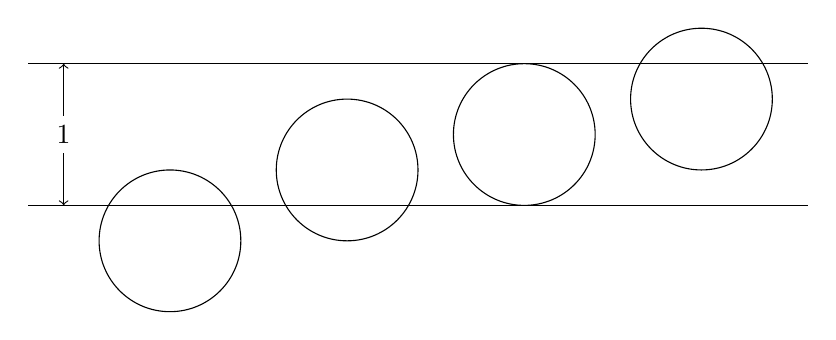
\begin{tikzpicture}[scale=.9]
\draw (0,0) -- (11,0);
\draw (0,2) -- (11,2);
\draw[<->] (.5,0) -- node[fill=white] {$1$} (.5,2);
\foreach \x/\y in {2/-.5, 4.5/.5, 7/1, 9.5/1.5}
  \draw (\x,\y) circle[radius=1];
\end{tikzpicture}
\end{center}
\caption{%
הפתרון של בעיית המחט של Buffon עם מעגלים}
\label{f.buffon3}
\end{figure}

תהי 
$E(x)$
התוחלת שמ מספר הקווים המקביליים שקו באורך
$x$
חוצה.

נתון מחט באורך
$a$
נשבור אותו למספר קטעים
$\{a_1,\ldots,a_n\}$
ולפי הליניאריות של התוחלת:
\[
E(a) = E\left(\sum_{i=1}^{n} a_i\right) = \sum_{i=1}^{n} E(a_i)\,, 
\]
ולכן לא משנה אם נחשב את התוחלת של כל קטע בנפרד. מכאן, שאם נכופף את המחט למעגל, התוחלת של מספר הקווים שהמעגל חוצה שווה למספר הקווים שהמחט חוצה.

נעיין בקו שמסובב למעגל
$C$
\textbf{בקוטר}
$1$
והיקף
$\pi$.
אם תזרוק את המעגל על המשטח הוא יחצה קו 
\textbf{בדיוק}
פעמיים (איור%
~\ref{f.buffon3}),
ולכן:
\begin{equation}\label{eq.buffon-2}
E(C)=2\,.
\end{equation}
בנה מצולע משוכלל
$Q_n$
חסום על ידי 
$c$
(אדום), ובנה מצולע משוכלל 
$R_n$
שחוסם את
$c$
(כחול) (איור%
~\ref{f.buffon4}). 
כל קו ש-%
$Q_n$
חוצה (אדום, מקווקו) חייב לחצות את המעגל וכל קו שחוצה את המעגל (כחול, מנוקד) חייב לחצות את 
$R_n$.
לכן:
\begin{equation}\label{eq.buffon3}
E(Q_n)\leq E(C)\leq E(R_n)\,.
\end{equation}
יהי 
$a_Q, a_R$
סכומי האורכים של צלעות של
$Q_n,R_n$,
בהתאמה. לפי הליניאריות של התוחלת:
{
\addtolength{\arraycolsep}{-3pt}
\begin{eqnarray}\label{eq.buffon1}
E(Q_n)&=&\sum_{i=1}^n E(a_Q\;\textrm{של צלעות})=a_QE(1)\\
\label{eq.buffon1b}E(R_n)&=&\sum_{i=1}^n E(a_R\;\textrm{של צלעות})=a_RE(1)\,. 
\end{eqnarray}
}
כאשר 
$n\rightarrow\infty$
שני המצולעים הם קירובים למעגל ולכן:
\begin{equation}\label{eq.buffon-pi}
\lim_{n\rightarrow\infty}a_Q = \lim_{n\rightarrow\infty} a_R=\pi\,,
\end{equation}
ההיקף של המעגל. ממשוואות%
~\ref{eq.buffon-pi}-\ref{eq.buffon1}
מתקבל:
\[
\renewcommand*{\arraystretch}{1.5}
\begin{array}{l}
\lim_{n\rightarrow\infty}E(Q_n)=E(C) =\lim_{n\rightarrow\infty}E(R_n)\\
E(C)=aE(1) =\pi E(1) = 2\\
E(1)=\disfrac{2}{\pi}\\
E(a)=aE(1)=\disfrac{2a}{\pi}\,.
\end{array}
\]
\begin{figure}[bt]
\begin{center}
\begin{tikzpicture}
\draw[thick,green!80!black] (0,0) circle[radius=2];
\node[draw,red,thick] (in)
  [minimum size=4cm,regular polygon,regular polygon sides=6]
  at (0,0) {};
\node[draw,blue,rotate=30,thick] (out)
  [minimum size=4.62cm,regular polygon,regular polygon sides=6]
  at (0,0) {};
\node[above left,xshift=5pt] at (in.corner 5) {$Q_n$};
\node[below right,yshift=6pt] at (out.corner 5) {$R_n$};
\draw[thick,red,dashed] (-3,-.6) -- +(6,0);
\draw[very thick,blue,dotted] (-3,1.85) -- +(6,0);
\end{tikzpicture}
\end{center}
\caption{מצולעים כקירובים למעגל}\label{f.buffon4}
\end{figure}

\sml{}

$\pi=2a/E$
ולכן ניתן לחשב קירוב לערכו על ידי הרצת סימולציה או זריקת מחטים על שולחן!
\selectlanguage{english}
\begin{verbatim}
For length = 0.2:
Expectation of crossings = 0.1273
Average crossings        = 0.1308
Empirical value for pi   = 3.0581

For length = 0.5:
Expectation of crossings = 0.3183
Average crossings        = 0.3227
Empirical value for pi   = 3.0989

For length = 1.0:
Expectation of crossings = 0.6366
Average crossings        = 0.6333
Empirical value for pi   = 3.1581
\end{verbatim}
\selectlanguage{hebrew}

%%%%%%%%%%%%%%%%%%%%%%%%%%%%%%%%%%%%%%%%%%%%%%%%%%%%%%%%%%%%%%%%

\begin{prob}{המחט של \L{Buffon} עם רשת אופקי ואנכי}{}{\\(Buffon's needle with horizontal and vertical rulings)}

פתור את בעיית המחט של 
\L{Buffon}
עבור משטח עם רשת אופקי ואנכי כאשר גודל המשבצות הוא 
$1\times 1$.
מחט יכול לחצות קו אנכי (כחול), קו אופקי (ירוק), שניהם (אדום) או אף אחד (כתום) (איור%
~\ref{f.buffon5}).

\begin{figure}[b]
\begin{center}
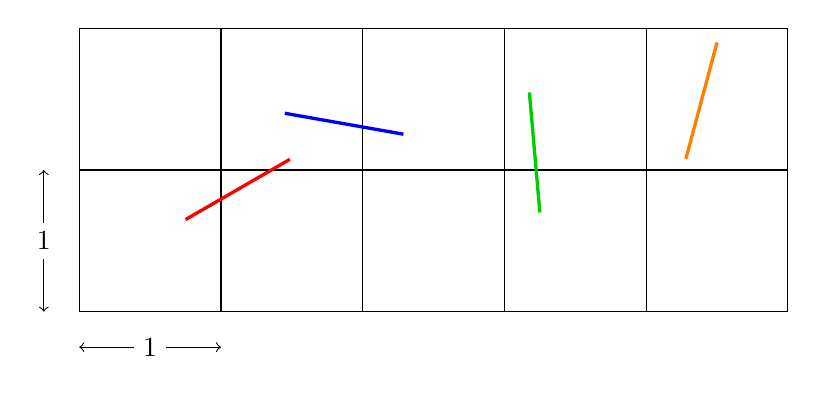
\begin{tikzpicture}[scale=.9]
\draw[step=2cm] (0,0) grid (10,4);
\draw[<->] (-.5,0) -- node[fill=white] {$1$} (-.5,2);
\draw[<->] (0,-.5) -- node[fill=white] {$1$} (2,-.5);
\foreach \x/\y/\a/\c in {
  1.5/1.3/30/red,
  2.9/2.8/-10/blue,
  6.5/1.4/95/green!80!black,
  9/3.8/-105/orange}
    \draw[color=\c,very thick] (\x,\y) -- +(\a:1.7);
\end{tikzpicture}
\end{center}
\caption{בעיית המחט של 
\L{Buffon}
עבור משטח עם רשת אופקי ואנכי}
\label{f.buffon5}
\end{figure}
\end{prob}
\textbf{רמז:}
האם מספר הקווים האופקים והקווים האכנים שהמחט חוצה בלתי-תלויים?

\solution{}

מספר הקווים האופקים והקווים האכנים שהמחט חוצה אכן בלתי-תלויים, ולפי הליניאריות של התוחלת:
\begin{eqn}
E(\textrm{חוצה}\; a\;\textrm{באורך שמחט קווים})&=&
E(\textrm{חוצה}\; a\;\textrm{באורך שמחט אנכים קווים}+\\
&&\quad\; \textrm{\textrm{חוצה}\; a\;\textrm{באורך שמחט אופקים קווים}})\\
&&E(\textrm{חוצה}\; a\;\textrm{באורך שמחט אנכים קווים})+\\
&&E(\textrm{\textrm{חוצה}\; a\;\textrm{באורך שמחט אופקים קווים}})\\
&=&\disfrac{2a}{\pi}+\disfrac{2a}{\pi}=\disfrac{4a}{\pi}\,.
\end{eqn}


%%%%%%%%%%%%%%%%%%%%%%%%%%%%%%%%%%%%%%%%%%%%%%%%%%%%%%%%%%%%%%%%

\begin{prob}{מחטים ארוכים}{D}{(Long needles)}

נתון מחט בבעיה של
\L{Buffon}
שאורכו
$a$
גדול מאחד.

\que{1}
מה התוחלת של
\textbf{מספר הקווים}
שמחט חוצה?

\que{2} 
פתח נוסחה עבור ההסתברות שהמחט חוצה
\textbf{לפחות קו אחד}?

\textbf{רמז:}
עבור איזו זוויות 
$\theta$
ההסתברות של חציית קו היא
$1$?

\end{prob}

\solution{}

\ans{1}
שבור את המחט לחלקים באורכים
$\{a_1,a_2,\ldots, a_n\}$, $a_i< 1$,
כך ש-%
$\sum_{i=1}^n a_i=a$.
בפתרון של בעיה%
~$53$
ראינו ש:
\[
E(a)= \sum_{i=1}^n E(a_i)= \disfrac{2a}{\pi}\,.
\]

\ans{2}
הפתרון מבוסס על
\L{\cite{wiki-buffon}}
ו-%
\L{\cite[Chapter~26]{proofs}}.

לפי משוואה%
~\ref{eq.cross}
ההסתברות שהמחט יחצה קו לפחות קו אחד היא
$a\sin\theta$ 
\textbf{אם}
$a\sin\theta \leq 1$,
כלומר, אם
$0\leq\theta\leq\sin^{-1}(1/a)$.
אולם אם
$a\sin\theta > 1$
ההסתברות היא
$1$
(איור%
~\ref{f.buffon6}).
נכליל את משוואה%
~\ref{eq.buffon-integral}
עבור
$a>0$
שרירותי על ידי חלוקת האינטגרל לשני חלקים, אחד עבור
$\theta<\sin^{-1}(1/a))$
ואחר עבור
$\theta>\sin^{-1}(1/a))$:
\begin{eqn}
E(a) &=& \disfrac{2}{\pi}
   \left(\int_{0}^{\sin^{-1}(1/a)} 
   a\sin \theta\:d\theta + 
   \int_{\sin^{-1}(1/a)}^{\pi/2} 1\: d\theta\right)\\
&=& \disfrac{2}{\pi}\left(\left.
    a(-\cos \theta)\right|_0^{\sin^{-1}(1/a)} + 
    \left(\disfrac{\pi}{2} - 
    \sin^{-1}(1/a)\right)\right)\\
&=& 1+\disfrac{2}{\pi}
  \left(a
  \left(1-\sqrt{1-\disfrac{1}{a^2}}\right)-
  \sin^{-1}(1/a)\right)\,.
\end{eqn}

\begin{figure}[tb]
\begin{center}
\begin{tikzpicture}[scale=1]
\draw (0,0) -- (10,0);
\draw (0,3.5) -- (10,3.5);
\draw[<->] (.5,0) -- node[fill=white,near end] {$1$} +(0,3.5);
\draw[<->] (5.5,0) -- node[fill=white] {$1/2$} +(0,1.75);
\begin{scope}[xshift=0cm,yshift=1.4cm,scale=1]
\coordinate (end1) at (2,-1);
\coordinate (end2) at ($(end1)+(60:3)$);
\coordinate (center) at ($(end1)+(60:1.5)$);
\node[above right,xshift=2pt,yshift=-2pt]
  at (end1) {$\theta$};
\draw (end1) --  node[left,near end] {$a/2$} (center) -- (end2);
\draw (end2) -- (end2 -| center);
\draw (end1) -- (end1 -| center);
\draw[very thick] (end1 -| center) -- 
  node[right,fill=white,yshift=2pt] {$(a/2)\sin \theta$}
  (center) -- (end2 -| center);
\draw[thick,dotted] (O |- center) -- +(10,0);
\end{scope}
\begin{scope}[xshift=3cm,yshift=.8cm,scale=1.6]
\coordinate (end1) at (2,-1);
\coordinate (end2) at ($(end1)+(60:3)$);
\coordinate (center) at ($(end1)+(60:1.5)$);
\node[above right,xshift=2pt,yshift=-2pt]
  at (end1) {$\theta$};
\draw (end1) --  node[left,near end] {$a/2$} (center) -- (end2);
\draw (end2) -- (end2 -| center);
\draw (end1) -- (end1 -| center);
\draw[very thick] (end1 -| center) -- 
  node[right,fill=white,yshift=6pt] {$(a/2)\sin \theta$}
  (center) -- (end2 -| center);
\end{scope}
\end{tikzpicture}
\end{center}
\caption{מחטים ארוכים}\label{f.buffon6}
\end{figure}

\sml{}
\selectlanguage{english}
\begin{verbatim}
For length = 1.5:
Expectation of crossings = 0.7786
Average crossings        = 0.7780
For length = 2.0:
Expectation of crossings = 0.8372
Average crossings        = 0.8383
For length = 3.0:
Expectation of crossings = 0.8929
Average crossings        = 0.8897
\end{verbatim}
\selectlanguage{hebrew}

%%%%%%%%%%%%%%%%%%%%%%%%%%%%%%%%%%%%%%%%%%%%%%%%%%%%%%%%%%%%%%%%

\begin{prob}{הכד של \L{Molina}}{}{(Molina's urns)}

שני כדים
$U_1,U_2$
מכילים 
$m$
כדורים כל אחד. ב-%
$U_1$
נמצאים 
$w_1$
כדורים לבנים ו-%
$b_1$
כדורים שחורים, וב-%
$U_2$
נמצאים
$w_2$
כדורים לבנים ו-%
$b_2$
כדורים שחורים. מכל כד שלוף
$n$
כדורים
\textbf{עם החזרה}.
עבור ערכים שונים של
$n>1$
מצא
$w_1,b_1,w_2,b_2$
כך ש:
\[
P(\textrm{לבנים}\;U_1\textrm{מ- שנשלפו כדורים כל})=
P(\textrm{שחורים או לבנים}\;U_2\textrm{מ- שנשלפו כדורים כל})\,.
\]
\end{prob}

\vspace{-8ex}

\solution{}

עבור 
$n=2$
המשוואה שיש לפתור היא:
\begin{eqn}
\left(\disfrac{w_1}{m}\right)^2&=&\left(\disfrac{w_2}{m}\right)^2+\left(\disfrac{b_2}{m}\right)^2\\
w_1^2&=&w_2^2+b_2^2\,,
\end{eqn}
וכל שלשת
\L{Pythagorean}
היא פתרון.

לפי המשפט האחרון של
\L{Fermat},
שהוכח ב-%
$1995$
על ידי
\L{Andrew Wiles},
אין פתרונות ל-%
$w_1^n=w_2^n+b_2^n$ 
עבור
$n\geq 3$.

\sml{}

הרצתי את הסימולציה עבור
$n=2$
ומספר שלשות
\L{Pythagorean}.

\selectlanguage{english}
\begin{verbatim}
For w1 = 17, w2 = 8, b2 =15:
Proportion of two whites in urn 1          = 0.5523
Proportion of two whites or black in urn 2 = 0.5387
For w1 = 29, w2 = 20, b2 =21:
Proportion of two whites in urn 1          = 0.5003
Proportion of two whites or black in urn 2 = 0.5026
For w1 = 65, w2 = 33, b2 =56:
Proportion of two whites in urn 1          = 0.5381
Proportion of two whites or black in urn 2 = 0.5384
\end{verbatim}
\selectlanguage{hebrew}

%%%%%%%%%%%%%%%%%%%%%%%%%%%%%%%%%%%%%%%%%%%%%%%%%%%%%%%%%%%%%%%%

